
%%%%%%%%%%%%%%%%%%%Reguläre Ausdrücke%%%%%%%%%%%%%%%%%%%%%%%%%
\section{Reguläre Ausdrücke}
\subsection*{}

\begin{frame}
  \frametitle{Definition}

  Reguläre Ausdrücke sind eine verbreitete und geeignete Notation, um reguläre
  Sprachen zu formalisieren.

	\begin{block}{Die Regeln (= Metazeichen)}
		\begin{tabular}{c p{0.7\textwidth}}
				\xb{Metazeichen} & 	\xb{Bedeutung} \\
				$( )$			& Klammerung von Alternativen\\
				$*$			& n-maliges Vorkommen\\
				$|$			& trennt Alternativen\\
		\end{tabular}
	\end{block}

  \begin{block}{Es gelten folgende Vorrangregeln:}
   \begin{itemize}
      \item $*$ bindet stärker als Verkettung
      \item Verkettung $(RS)$ bindet stärker als "`oder"' $(R|S)$
      \item Überflüssige Klammern dürfen wir weglassen. \\
      So sind $(RS),((RS)),\ldots$ und $RS$ äquivalent
    \end{itemize}
  \end{block}
\end{frame}


\subsection*{}
\begin{frame}
  \frametitle{Definition}
	\begin{block}{Die Sprache von R}
		Wenn \textbf{R} ein regulärer Ausdruck ist, dann bezeichnen wir mit \textbf{$\langle R \rangle$} die Sprache, die dieser erzeugt.\\
  		\begin{itemize}
    			\item $\langle \emptyset \rangle =\{\}$
			\item Für $a \in A$ ist $\langle a \rangle=\{a\}$
			\item $\langle R_1 | R_2 \rangle = \langle R_1 \rangle \cup \langle R_2 \rangle$
			\item $\langle R_1 R_2 \rangle = \langle R_1 \rangle \cdot \langle R_2 \rangle$
  		\end{itemize}
	$R_1$ und $R_2$ sind hier zwei beliebige reguläre Ausdrücke.


	\end{block}
\end{frame}

\subsection*{}
\begin{frame}
  \frametitle{Die Sprache von R}
	\begin{block}{Beispiel 1}
		Welche Wörter erzeugt der folgende reguläre Ausdruck R?
  		\begin{itemize}
			\item $R=(a|b)*abb(a|b)*$ ? \pause
			\item $\langle R \rangle$ enthält genau die Wörter, in denen das Teilwort $abb$ vorkommt.
  		\end{itemize}
	\end{block}

	
	\begin{block}{Beispiel 2}
		Gebe einen regulären Ausdruck für die Sprache aller Wörter die nicht $ab$
		enthalten
  		\begin{itemize} \pause
			\item $ {b*} {a*}$
  		\end{itemize}
	\end{block}
	
\end{frame}

\subsection*{}
\begin{frame}
  \frametitle{Die Sprache von R}
	\begin{block}{Beispiel 3}
		Welcher reguläre Ausdruck R erzeugt die Sprache $\{\epsilon\}$?
  		\begin{itemize}
			\visible<2->{\item $\emptyset*$, denn $\langle \emptyset \rangle ^* =
			\{\}^* = \{\epsilon\}$}
  		\end{itemize}
	\end{block}

	\visible<3->{
	\begin{block}{Beispiel 4}
		Gebe einen regulären Ausdruck für die Sprache aller Wörter mit mindestens 3 b's an!
  		\begin{itemize}
			\visible<4->{\item $(a|b)*b(a|b)*b(a|b)*b(a|b)*$ oder
			\visible<5->{\item $a*ba*ba*b(a|b)*$}}
  		\end{itemize}
	\end{block}
	}
\end{frame}

%%%%%%%%%%%%%%%%%%%Rechtslineare Grammatiken%%%%%%%%%%%%%%%%%%%%%%%%%
\section{Rechtslineare Grammatiken}

\subsection*{}
\begin{frame}
	\frametitle{rechtslineare Grammatiken}
	\begin{block}{etwas genauer...}
  		Eine rechtslineare Grammatik ist eine kontextfreie Grammatik $G=(N,T,S,P)$ mit folgenden Einschränkungen. Jede Produktion ist entweder von der Form
  		\begin{itemize}
			\item $X \rightarrow w$ oder
			\item $X \rightarrow wY$ mit $w \in T^*$ und $X,Y \in N$
  		\end{itemize}
	\end{block} \pause

	\begin{block}{Regex}
    Zu jeder rechtslinearen Grammatik gibt es:
		\begin{itemize}
			\item \ldots einen entsprechenden regulären Ausdruck und \pause
			\item \ldots einen einen deterministischen endlichen Automaten
        \end{itemize}
    Zu jeder rechtslinearen gibt es äquivalente linkslineare Grammatiken. Diese
    "`können"' nichts anderes als rechtslineare Grammatiken, daher ignorieren
    wir sie in dieser Vorlesung.
	\end{block}
\end{frame}


\subsection*{}
\begin{frame}
	\frametitle{rechtslineare Grammatiken}
	\begin{block}{Ein Beispiel \only<2->{- oder auch nicht...}}
  		Gegeben Sei die Grammatik $G=(\{X,Y\},\{a,b\},X,\{X \rightarrow aY | \epsilon, Y \rightarrow Xb\})$\\
  		\begin{itemize}
  		\item Ist diese Grammatik rechtslinear? \\
		\visible<2->{$G$ ist offensichtlich nicht rechtslinear, denn die Produktion $Y \rightarrow Xb$ hat das Nichtterminalsymbol links vom Terminalsymbol \\
		(Die Produktion ist linkslinear)!\\
		\visible<3->{\item Die Grammatik erzeugt die Sprache $L(G)=\{a^k b^k | k \in \mathbb N_0 \}$}\\}
		\visible<4->{\item Kann es eine rechtslineare Grammatik für diese Sprache
		geben? \\ Ist diese Sprache regulär? \\ } 
		\visible<5->{ Nein, ist sie nicht! }
		\end{itemize}
	\end{block}
\end{frame}

\subsection*{}

\begin{frame}
\frametitle{von G zu L(G)}
	\begin{block}{Aufgabe}
		Betrachte $G=(\{X,Y,Z\},\{a,b\},X,P)$ mit $P=\{X \rightarrow aX | bY | \epsilon, Y \rightarrow aX | bZ | \epsilon, Z \rightarrow aZ | bZ \}$
  		\begin{itemize}
			\item Was ist $L(G)$?
			\item Geben Sie einen endlichen Automaten an, der L(G) akzeptiert.
			\item Lässt sich diese Grammatik noch vereinfachen?
  		\end{itemize}
	\end{block}
	\visible<2->{
	\begin{block}{Lösung}
      		\begin{tikzpicture}[shorten >=1pt,node distance=2cm,auto,initial text=,>=stealth]
        		\node[state,initial,accepting]  (q_0)                       {$0$};
       			\node[state,accepting]          (q_1) [right of= q_0] {$1$};
        		\node[state]                    (q_2) [right of= q_1] {$2$};
        		\path[->] (q_0) edge [loop below]      node        {$a$} ()
        		edge [bend right] node [swap] {$b$} (q_1)
        		(q_1) edge              node        {$b$} (q_2)
        		edge [bend right] node [swap] {$a$} (q_0)
        		(q_2) edge [loop below] node        {$a,b$} ()
        		;
      		\end{tikzpicture}
	\end{block}
	}
\end{frame}

\begin{frame}
	\frametitle{Ist doch alles das Gleiche, oder?}
	\begin{block}{Gleiche Sprache - andere Grammatik}
	Folgende Grammatiken erzeugen die gleiche Sprache
  	\begin{itemize}
    		\item $G=(\{X,Y,Z\},\{a,b\},X,P)$ mit $P=\{X \rightarrow aX | bY | \epsilon, Y \rightarrow aX | bZ | \epsilon, Z \rightarrow aZ | bZ \}$
		\visible<2->{\item $G=(\{X,Y\},\{a,b\},X,P)$ mit $P=\{X \rightarrow a X | b Y | \epsilon, Y \rightarrow aX | \epsilon \}$
		\visible<3->{\item $G=(\{X\},\{a,b\},X,P)$ mit $P=\{X \rightarrow aX | baX |
		b | \epsilon \}$}}
  	\end{itemize}
  	\end{block}
\end{frame}


\section[Bäume]{Kantorowitsch-Bäume, Regex-Bäume}

\subsection*{}
\begin{frame}
	\frametitle{Kantorowitsch-Bäume, Regex-Bäume}
	\begin{block}{Kantorowitsch}
	Beispiel: 
  	\begin{itemize}
        \item wie sieht der Baum zu $3+(a+b)*(-c)$ aus? \pause
        \item wie hoch ist der Baum? \pause Antwort: $3$
      \end{itemize} \pause
      Die Höhe eines Baumes entspricht auch dem längsten wiederholungsfreien
      Weg von der Wurzel zu den Blättern.
  	\end{block}

	\begin{block}{Kantorowitsch-Bäume zu Reg. Ausdrücken} \pause
	\begin{itemize}
        \item Wird ein regulärer Ausdruck als Baum dargestellt, sind Klammern auch
        unnötig \pause
        \item durch die "`Eltern-Kind"'- bzw. "`ist-Teilausdruck"'-Beziehung im
        Baum ist die Klammerung eindeutig festgelegt 
        \end{itemize}
  	\end{block}
\end{frame}






%vielleicht noch ein paar praktische Fragen nach Berechenbarkeit (mir fällt da grad nur das Rundreiseproblem ein)
%%%%%%%%%%%%%%%%%%%Berechenbarkeit%%%%%%%%%%%%%%%%%%%%%%%%%
\section{Berechenbarkeit}
\subsection*{}
\begin{frame}
  \frametitle{}

	\begin{block}{Typische Fragestellung}
\begin{itemize}
 	\item Gibt es Aufgaben, die von einem Rechner unabhängig
 		\begin{itemize}
       			\item von der Art der Programmierung
       			\item von physikalischen und elektronischen Beschränkungen
   		\end{itemize}
	\item nicht gelöst werden können?
	\item \textbf{Hauptfrage:} Welche Probleme sind dann berechenbar?
\end{itemize}
	\end{block}
	\pause
  \begin{block}{Lösungsansätze}
  Entwicklung neuer Konzepte wie
   \begin{itemize}
      \item eine grundlegende \textbf{Problemformulierung}
      \item ein grundlegendes \textbf{Rechnermodell}
    \end{itemize}
    Dafür muss geklärt werden wie ein Rechner (der nur \emph{Nullen} und \emph{Einsen} kennt) ein Problem überhaupt löst.
  \end{block}
\end{frame}


\subsection*{}
\begin{frame}
  \frametitle{Suche nach Rechnermodell}
  \pause
  \begin{block}{Vorschlag}
    \textbf{endliche Automaten} als Grundlage für "`allgemeine"' theoretische Aussagen über "`Berechenbarkeit"'
   \end{block}
    \pause
   \begin{block}{Problem}
    \begin{itemize}
      \item nicht mächtig genug!
      \item es ist zwar erfassbar, ob ein Getränkeautomat (wie aus der Vorlesung) eine Eingabe verabeiten kann, ABER das Modell wäre spätestens bei kontextsensitiven Sprachen überfordert
    \end{itemize}
  \end{block}
\pause
\textbf{Frage:} Gibt es ein mächtigeres, realistisches Rechnermodell, das geeignet ist?\end{frame}

%%%%%%%%%%%%%%%%%%%%%%%%%%%%%% Turingmaschinen %%%%%%%%%%%%%%%%%%%%
\section{Turingmaschinen}

\subsection*{}
\begin{frame}
  \frametitle{Aufbau der Turing-Maschine}
  Erfinder: Alan Turing (1936)
  \pause
	\begin{block}{Bestandteile} % ANZEICHNEN!!!
  	\begin{itemize}
      \item beidseitig unendliches Eingabe- und Rechenband
			\item freibeweglicher Lese-/Schreibkopf
			\item gesteuert von einer endlichen Kontrolle
  	\end{itemize}
	\end{block}
	\pause
	\begin{block}{Eigenschaften}
  	\begin{itemize}
	      	\item Eingabe- und Rechenband enthält eine Folge von Symbolen
			\item Kontrolle ist in einem von endlich vielen Zuständen
			\item Zellen des Bandes enthalten jeweils höchstens ein Symbol aus dem Bandalphabet
  	\end{itemize}
	\end{block}
\end{frame}

\subsection*{}
\begin{frame}
\frametitle{Funktionsweise}
	\begin{block}{So arbeitet die TM}
	Ist die Turing-Maschine (TM) in einem bestimmten Zustand und liest ein Symbol...
\begin{itemize}
	\item 	so geht sie in einen Folgezustand über
	\item 	überschreibt eventuell das Symbol und
	\item 	bewegt den Lese-/Schreibkopf eine Stelle nach rechts, nach links oder überhaupt nicht
\end{itemize}
\end{block}
\end{frame}

\subsection*{}
\begin{frame}
  \frametitle{Definition der TM}

  \begin{block}{Ganz genau}
    Eine Turingmaschine $T = (Z, z_0, X, f, g, m)$ ist festgelegt durch
\begin{itemize}
	\item eine endliche \textbf{Zustandsmenge} $Z$
	\item einen \textbf{Anfangszustand} $z_0 \in Z$
	\item ein endliches \textbf{Bandalphabet} $X$
	\pause
	\item eine partielle \textbf{Zustandsüberführung}sfunktion $f : Z \times X \dashrightarrow  Z$
	\item eine partielle \textbf{Ausgabe}funktion $g : Z \times X \dashrightarrow  X$ und
	\item eine partielle \textbf{Bewegung}sfunktion $m : Z \times X \dashrightarrow  \{-1, 0, 1\}$\end{itemize}
\end{block}
\end{frame}

\subsection*{}
\begin{frame}
  \frametitle{Definition der TM}

  \begin{block}{Anmerkungen}
\begin{itemize}
	\item Die Funktionen \textbf{f}, \textbf{g} und \textbf{m} beschreiben, wie das eingelesene Zeichen verarbeitet werden soll (gemeinsamer Definitionsbereich)
		\pause
	\item Bei der Bewegungsfunktion bedeutet \textbf{-1 oder L} eine Bewegung des Lese-/Schreibkopfes nach links, \textbf{1 oder R}
eine Bewegung nach rechts und \textbf{0 oder N} ein Stehenbleiben\pause
  \item Im Bandalphabet gibt es ein sogenanntes Blanksymbol  $\square \in X$ zur Beschreibung einer leeren Zelle auf dem Band
  \item ein endliches Eingabealphabet $ A \subset X \setminus \{\square\}$
  \item eine endliche Menge von akzpetierenden Zuständen $F \subseteq Z$
\end{itemize}
\end{block}
\end{frame}

\subsection*{}
\begin{frame}
  \frametitle{Konfiguration einer TM}
Eine Turingmaschine befindet sich zu jedem Zeitpunkt in einem \textit{Gesamtzustand}, der als \textbf{Konfiguration} $(z, b, p) \in Z \times X^\mathbb{Z} \times \mathbb{Z}$ bezeichnet wird
\begin{block}{Vollständig beschrieben durch...}
\begin{itemize}
  \pause
	\item den aktuellen \textbf{Zustand} $z \in Z$ der Steuereinheit,
	\pause
	\item die aktuelle \textbf{Beschriftung des gesamten Bandes}, die man als Abbildung $b: \mathbb{Z} \rightarrow X$ formalisieren kann, und
	\pause
	\item die aktuelle \textbf{Position} $p \in Z$ \textbf{des Kopfes}.
\end{itemize}
\end{block}
\end{frame}

\subsection*{}
\begin{frame}
  \frametitle{Beispiele}
\begin{block}{Einfach I}
\begin{figure}
	\centering
           \begin{tikzpicture}[shorten >=1pt,initial text=,node distance=1.5cm,auto,->,>=stealth,baseline=(B.base)]
             \node[state,initial]  (S)          {$q_1$};
             % \node (nix) [right of=A] {};
             \node[state]          (B) [right of=S, node distance=2.5cm] {$q_2$};

             \path[->]
             %(S) edge              node  {$$\square$\io$\square$R$} (A)
             (S) edge              node  {$a | b, R$} (B)
             ;
           \end{tikzpicture}


\end{figure}
\end{block}
\pause
 \begin{block}{Bedeutung des Übergangs}
 Ist die TM im Zustand $q_1$ und liest das Sysmbol a, so überschreit sie dieses a mit b, geht auf dem Bande eine Stelle nach rechts und wechselt in den Zustand $q_2$
\end{block}
\end{frame}

\subsection*{}
\begin{frame}
  \frametitle{Beispiel}
      \begin{center}
           \begin{tikzpicture}[shorten >=1pt,initial text=,node distance=1.5cm,auto,->,>=stealth,baseline=(B.base)]
             %\node[state,initial]  (S)                       {$S$};
             \node[state,initial]  (A)          {$A$};
             % \node (nix) [right of=A] {};
             \node[state]          (B) [above right of=A] {$B$};
             \node[state]          (C) [right of=B, node distance=2.5cm] {$C$};
             \node[state]          (E) [below right of=A] {$E$};
             \node[state]          (D) [right of=E, node distance=2.5cm] {$D$};


             \path[->]
             %(S) edge              node  {$$\square$\io$\square$R$} (A)
             (A) edge              node  {$1 | X R$} (B)
             (B) edge [loop above] node  {$1 | 1 R$} ()
             edge              node  {$\square | \square R$} (C)
             (C) edge [loop above] node  {$ 1 | 1 R$} ()
             edge              node  {$\square | 1 L$} (D)
             (D) edge [loop below] node  {$ 1 | 1 L$} ()
             edge              node  {$\square | \square L$} (E)
             (E) edge [loop below] node  {$ 1 | 1 L$} ()
             edge              node  {$ X | 1 R$} (A)
             % (B) edge              node        {$\square$\io$\square$R$} (B)
             % edge [loop right] node        {$1$\io$1$R$} ()
             % (B) edge [loop right] node {$\square$\io$1$L$} ()
             % edge  node [pos=0.3]       {$1$\io$1$L$} (A)
             ;
           \end{tikzpicture}
   				\begin{tabular}[t]{c|>{$}c<{$}@{\qquad}*{5}{c}}
            & A       & B      & C       & D       & E \\
            \hline
    		$\square$  &  & $\square$,R,C & 1,L,D & $\square$,L,E  &  \\
            1         & X,R,B & 1,R,B& 1,R,C & 1,L,D & 1,L,E \\
            X         &         &        &        &         & 1,R,A \\
          \end{tabular}
      \end{center}
\end{frame}

\subsection*{}
\begin{frame}
  \frametitle{Verhalten von TM bei Entscheidungsproblemen}
\begin{block}{akzeptierende Zustände}
Eine Turing-Maschine akzeptiert eine Eingabe $w$, wenn sie nach Lesen
von $w$ in einem akzeptierenden Zustand $F \subset Z$ stoppt. \\
Es gibt Eingaben, für die eine Turing-Maschine unter Umständen niemals
stoppt, bzw. nur in einem nicht akzeptierenden Zustand.
\end{block} \pause
\begin{block}{Terminierung}
Wann terminiert eine TM? \\ \pause
\textbf{Wenn der nächste Schritt nicht mehr definiert ist.}
\end{block}
\end{frame}


\subsection*{}
\begin{frame}
	\frametitle{Ihr seid dran...}
	\only<1>{
	\begin{block}{Aufgabe}
	Gebt die Berechnung der folgenden Turingmaschine für die Eingaben
	\begin{enumerate}
		\item aba
		\item baba
	\end{enumerate}
	\end{block}}
\only<2->{
\begin{figure}
	\centering
		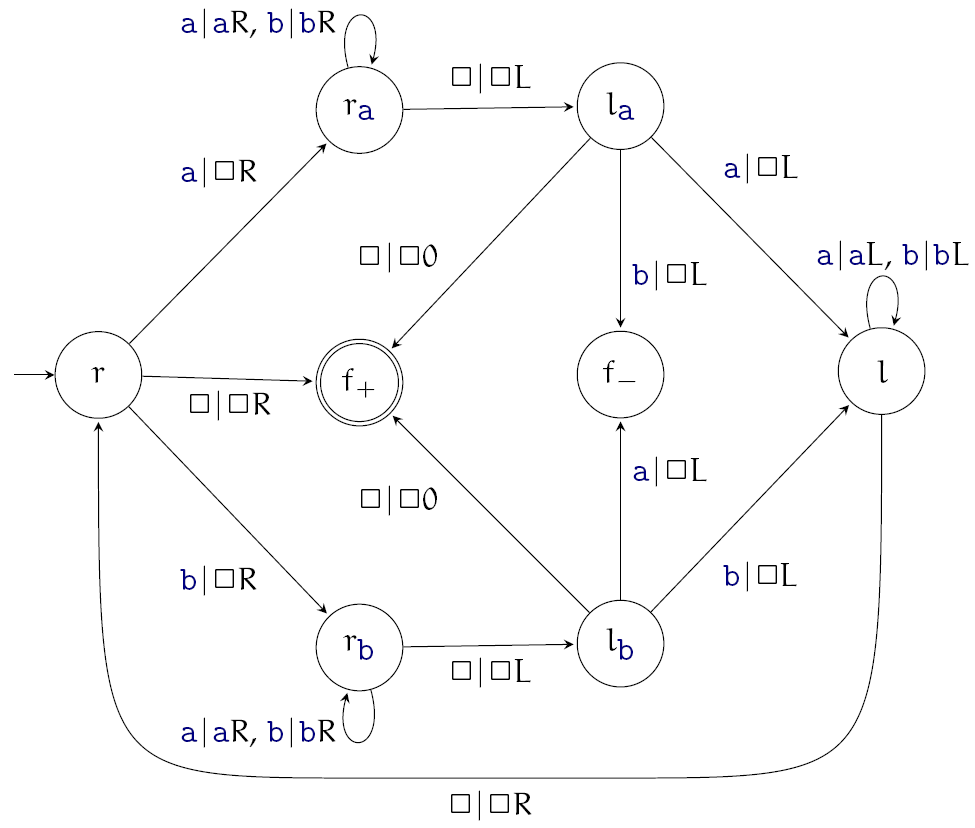
\includegraphics[height=7cm]{src/tut12_palindromturing}
\end{figure}}
\end{frame}

\subsection*{}
\begin{frame}
  \frametitle{Ihr seid dran...}

  \begin{block}{Aufgabe}
	Gebt eine Turingmaschine an die alle Wörter aus $\{0,1\}^*$ erkennt, die mit einer Eins beginnen
	\end{block}
  \only<2->{
\begin{block}{Lösung (nicht minimal)}
	\centering
           \begin{tikzpicture}[shorten >=1pt,initial text=,node distance=2.5cm,auto,->,>=stealth,baseline=(C.base)]
             \node[state,initial]  (S)          {$S$};
             % \node (nix) [right of=A] {};
             \node[state]          (B) [above right of=S] {$q_1$}; %
             \node[state, accepting]   (C) [below right of=S] {$q_2$};


             \path[->]
             %(S) edge              node  {$$\square$\io$\square$R$} (A)
             (S) edge [loop below] node  {$\square | \square, R$} ()
             edge   [bend above]           node  {$0 | 0, R$} (B)
             edge    [bend below] node  {$1 | 1, R$} (C)
%             edge              node  {$\square | 1 L$} (D)
%             (D) edge [loop below] node  {$ 1 | 1 L$} ()
%             edge              node  {$\square | \square L$} (E)
%             (E) edge [loop below] node  {$ 1 | 1 L$} ()
%             edge              node  {$ X | 1 R$} (S)
             % (B) edge              node        {$\square$\io$\square$R$} (B)
             % edge [loop right] node        {$1$\io$1$R$} ()
             % (B) edge [loop right] node {$\square$\io$1$L$} ()
             % edge  node [pos=0.3]       {$1$\io$1$L$} (A)
             ;
           \end{tikzpicture}



\end{block}}\end{frame}


\subsection*{}
\begin{frame}
  \frametitle{partielle Funktion von TM}
\begin{block}{Eine TM kann mehr...}
Eine Turing-Maschine erkennt nicht nur Mengen von Wörtern (Sprachen), sondern sie verändert auch die Eingabe und hat insofern auch eine
Ausgabe (= Inhalt des Bandes nach der Bearbeitung).\\
Eine TM kann so zur Berechnung von Funktionen genutzt werden, wie der Addition oder dem Vergleich zweier Binärzahlen
\end{block}
\end{frame}

\begin{frame}
	\frametitle{Wir konstruieren eine solche TM...}

	\begin{block}{Ihr seid dran...}
	Gebt eine Turing-Maschine an, die eine in Binärcodierung gegebene natürliche Zahl $n\geq 1$
mit der Zahl $2$ multipliziert. Der Schreib-/Lesekopf soll sich zu Anfang und Ende der Berechnung
jeweils auf dem ersten Bit (der größten Zweierpotenz zugeordnet) der Darstellung von
n befinden...
	\end{block}
	\visible<2>{
			\begin{block}{Lösung}
	     \begin{center}
       \begin{tikzpicture}[shorten >=1pt,initial text=,node distance=2.5cm,auto,->,>=stealth,baseline=(B.base)]
        	\node[state,initial]  (A)         						{$A$};
					\node[state]					(B)[right of=A]					{$B$};
					\node[state]					(C)[right of=B]					{$C$};

					\path[->]
					(A) edge [loop above] node  {$1 | 1 R$,$0 | 0R$} ()
							edge							node	{$\square | 0L$} (B)
					(B) edge [loop above] node  {$1 | 1 L$,$0 | 0L$} ()
							edge							node	{$\square | \square R$} (C);

				\end{tikzpicture}
				\end{center}
				\end{block}}
\end{frame}

\subsection*{}
\begin{frame}
  \frametitle{Entscheidbarkeit und Berechenbarkeit}
\begin{block}{Die "`verschiedenen Arten"' von TMs}
Verknüpfung von Entscheidbarkeit von Sprachen und der Berechenbarkeit
von Funktionen:

\begin{itemize}
	\item Eine Turing-Maschine akzeptiert eine Sprache L, wenn sie genau für die Eingaben $w \in L$ stoppt.
	\item L ist entscheidbar, wenn es eine Turing-Maschine gibt, die auf allen Eingaben stoppt und L akzeptiert.
	\item Die Funktion f heißt berechenbar, wenn eine Turing-Maschine existiert, die f realisiert.
\end{itemize}
\end{block}
\end{frame}


\subsection*{}
\begin{frame}
  \frametitle{Berechnungsschritt, d.h. Konfigurationswechsel}
  \pause
  Die \textbf{Menge aller Konfigurationen} bezeichnen wir als $\mathbb{C}_t$
  \pause
  \begin{block}{Schritt einer TM}
\begin{itemize}
	\item   $\Delta_x : \mathbb{C}_t \dashrightarrow  \mathbb{C}_t$
  \item		$\Delta_1(c)$ liefert direkte Nachfolgekonfiguration zu c
\end{itemize}
  \end{block}
  \pause
    \begin{block}{Endkonfigurationen einer TM}
  ist erreicht, falls $\Delta_1(c)$ nicht definiert ist
  \end{block}
\end{frame}

\subsection*{}
\begin{frame}
  \frametitle{Arten der Berechnung}

  \pause
  \begin{block}{endliche Berechnung}
\begin{itemize}
	\item endliche Folge von Konfigurationen $(c_0, c_1, c_2, . . . , c_t )$,
	\item wobei $0 < i \leq t$ gilt  $c_i = \Delta_1(c_{i-1})$
\end{itemize}
  \end{block}

  \pause
  \begin{block}{haltende Berechnung}
\begin{itemize}
	\item endliche Berechnung
	\item deren letzte Konfiguration eine Endkonfiguration ist
\end{itemize}
  \end{block}

  \pause
  \begin{block}{unendliche Berechnung}
\begin{itemize}
	\item unendliche Folge von Konfigurationen $(c_0, c_1, c_2, . . . )$
	\item wobei $0 < i$ gilt  $c_i = \Delta_1(c_{i-1})$
	\item \textbf{nicht haltend}
\end{itemize}
  \end{block}
\end{frame}

\subsection*{}
\begin{frame}
  \frametitle{Turingmaschinenakzeptoren}
  \pause
  \begin{block}{analog zu endlichen Automaten}
\begin{itemize}
	\item   \textbf{Erkennung formaler Sprachen}: ein Bit akzeptiert/abgelehnt
	\pause
  \item		Teilmenge $F \subset Z$ \textbf{akzeptierender Zustände}
  \item		TM akzeptiert Eingabewort $w$, wenn
\begin{itemize}
	\pause
	\item TM für Eingabe $w$ hält und
	\pause
	\item der Zustand der Endkonfiguration $\Delta_{*}(c_0(w))$ akzepierend ist
\end{itemize}
\pause
\item $L(T)$: Menge der akzeptierten Wörter
\end{itemize}
\end{block}
\end{frame}

\subsection*{}
\begin{frame}
  \frametitle{Ihr seid dran...}
	\only<1>{
  \begin{block}{Aufgabe}
	Gebt ein TM-Akzeptor an, der die Sprache $L^= = \{0^n1^n : n \geq 1\}$ akzeptiert
	\end{block}}
  \only<2->{
\begin{block}{Lösung (die Markierung des Startzustands fehlt)}
\begin{figure}
	\centering
		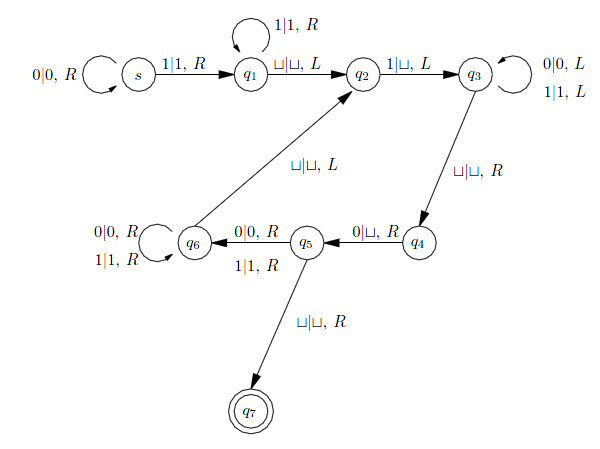
\includegraphics[height=6.7cm]{src/tut13_tmaufgabe.png}
\end{figure}
\end{block}}
\end{frame}

\subsection*{}
\begin{frame}
  \frametitle{Aufzählbare und entscheidbare Sprachen}
  \begin{block}{zwei Möglichkeiten, wenn $w$ von TM nicht akzeptiert wird}
\begin{enumerate}
\pause
	\item TM hält für Eingabe $w$, aber Endzustand nicht akzeptierend
	\pause
  \item	TM hält für Eingabe $w$ \textbf{nicht}
\end{enumerate}
\end{block}
\pause
  \begin{block}{Was wissen wir über die Berechnung?}
\begin{enumerate}
\pause
	\item TM ist fertig und lehnt die Eingabe ab
\pause
  \item	TM ist noch nicht fertig (\textit{Ob TM irgendwann w noch akzeptiert oder ablehnt, ist unklar!})
\end{enumerate}
\end{block}
\pause
  \begin{block}{Wir halten in zwei Definitionen fest}
\begin{enumerate}
	\item $L$ heißt \textbf{entscheidbare Sprache}, wenn es eine TM gibt, die \textbf{immer hält} und $L$ akzeptiert.
	\pause
	\item $L$ heißt \textbf{aufzählbare}(semi-entscheidbar) \textbf{Sprache}, wenn es eine TM gibt, die $L$ akzeptiert
\end{enumerate}
\end{block}
\end{frame}


\section{Abschluss}
% Studis anzuregen darüber nachzudenken, ob sie wirklich alles wissen, ansonsten nachlesen oder fragen nachträglich stellen, dann kann in der nächsten Woche nochmal drauf eingegangen werden
\subsection*{}
\begin{frame}
	\frametitle{Zum Schluss...}
	\begin{block}{Was ihr nun wissen solltet!}
	\begin{itemize}
	  	\visible<2->{\item Was verstehen wir unter Berechenbarkeit?}
		\visible<3->{\item Welches Rechenmodell ist in der Informatik von zentrale Bedeutung?}
		\visible<4->{\item Was sind die Bestandteile dieses Rechenmodells? Und wie arbeitet es?}
		\visible<5->{\item Was lässt sich aus diesem Rechenmodell ableiten?}
		\visible<6->{\item Wann ist eine Sprache entscheidbar?}
    \end{itemize}
   	\end{block}

	\visible<7->{
	\begin{block}{Ihr wisst was nicht?}
		Stellt \textbf{jetzt} Fragen!
	\end{block}}
\end{frame}